\documentclass[a4paper]{article}
\usepackage[utf8]{inputenc}
\usepackage[spanish]{babel}

\usepackage{xcolor}     % \textcolor
\usepackage{amsmath}    % 
\usepackage{caratula}   % caratula del TP
\usepackage{url}



\usepackage[ruled,noline]{algorithm2e}
\usepackage{subcaption}

% Figuras y graficos
\usepackage{float}
\usepackage{graphicx}
\usepackage{pgfplotstable}

% Tablas
\usepackage{xltabular}

\usepackage{amssymb}
\usepackage{hyperref}
 
\newcommand{\norm}[1]{\left\lVert#1\right\rVert}%
\newcommand{\pint}[1]{\left\langle#1\right\rangle}%
\newcommand{\fss}{\emph{forward stepwise selection}}
\newcommand{\cv}{\emph{cross validation}}
\newcommand{\fe}{\emph{feature engineering}}

\providecommand{\keywords}[1]
{
  \small	
  \textbf{\textit{Keywords---}} #1
}

% ********************************************************* %
% ~~~~~~~~         Formato de las páginas         ~~~~~~~~~ %
% ********************************************************* %

\usepackage{csquotes}
\usepackage{fancyhdr}
\pagestyle{fancy}

%\renewcommand{\chaptermark}[1]{\markboth{#1}{}}
\renewcommand{\sectionmark}[1]{\markright{\thesection\ - #1}}

\fancyhf{}

\fancyhead[LO]{Sección \rightmark} % \thesection\ 
\fancyfoot[RO]{\thepage}
\renewcommand{\headrulewidth}{0.5pt}
\renewcommand{\footrulewidth}{0.5pt}
\setlength{\hoffset}{-0.8in}
\setlength{\textwidth}{16cm}
%\setlength{\hoffset}{-1.1cm}
%\setlength{\textwidth}{16cm}
\setlength{\headsep}{0.5cm}
\setlength{\textheight}{25cm}
\setlength{\voffset}{-0.7in}
\setlength{\headwidth}{\textwidth}
\setlength{\headheight}{13.1pt}
\renewcommand{\baselinestretch}{1.1}  % line spacing

%**********************************************************%




\begin{document}

\thispagestyle{empty}
\materia{Métodos Numericos}
\submateria{Primer Cuatrimestre de 2020}
\titulo{Trabajo Práctico 3}
\subtitulo{Metros cuadrados mínimos lineales} % Literal se llama así el TP WeirdChamp tenia que ponerle el nombre real LMAO
\integrante{Manuel Panichelli}{72/18}{panicmanu@gmail.com}
\integrante{Tomas Tropea}{115/18}{tomastropeaa@gmail.com}
\integrante{Ignacio Alonso Rehor}{195/18}{arehor.ignacio@gmail.com}

\maketitle
\newpage

\thispagestyle{empty}
\tableofcontents

% Objetivos generales

\newpage 

\section{Abstract}

En este trabajo se estudia el método de \emph{Least squares} (o cuadrados mínimos lineales) aplicado a la predicción de características de inmuebles del mercado mexicano. Proponemos distintos modelos de regresiones, como pueden ser lineales o polinomiales; introducimos el concepto de segmentación del conjunto de datos, por características como el tipo de propiedad, o la antiguedad de la propiedad; y también construimos nuevas características a partir de las que ya presentes (\textit{feature engineering}).

Concluimos que para su simpleza, los regresores empleados tienen buenos resultados medidos con distintas métricas, por ejemplo r2, para la predicción de precio (r2 = 0.54) y en especial metros cubiertos (r2 = 0.70) de un inmueble.

\keywords{least squares, cml, statistical analysis, predictive models, cross validation, feature engineering}


\section{Introducción}

La capacidad de predecir el comportamiento de ciertos fenómenos que nos rodean es de gran interés en muchos ámbitos. Ejemplos de estos fenómenos incluyen la meteorología o el análisis financiero, entre otros. Uno puede formalizar estas ideas, y plantear este problema como, dado un conjunto de variables independientes (a las cuales se las conoce como features o predictores), estimar una variable dependiente. Sobre este concepto se construye lo que se conoce como \textbf{Regression Analysis}. Esta busca estimar las relaciones entre una variable dependiente (la que se quiere predecir) y una o más variables independientes (los predictores), lo que se busca con este tipo de análisis es poder inferir relaciones entre las variables observacionales.

Para llevar a cabo el análisis por regresión se debe construir un modelo de regresión, que puede ser muy simple, o involucrar cosas mas sofisticadas. Un caso simple de regresión es el de una regresión lineal, que involucra una función lineal, o por otro lado, una regresión mas compleja que involucra polinomios, funciones logarítmicas o exponenciales. 

Una vez que se tiene decidido el tipo de modelo a utilizar, se lo debe ``ajustar" (fitting) lo mejor posible a los datos para que los describa de la mejor manera posible. Esto ultimo puede hacerse, por ejemplo, a través del método de CML (Cuadrados Mínimos Lineales).

Nuestro objetivo fue aplicar \textit{Regression Analysis} sobre datos de inmuebles, y en particular, establecer una relación entre el precio y las características de la propiedad, como la cantidad de habitaciones, baños, sus metros cubiertos, etc. Comparamos distintos modelos, como regresor lineal y polinomial, bajo distintas métricas, para ver que opción era mejor, utilizando el método de CML para el fitting de los mismos.

\section{Metodologia}

\subsection{Modelos de regresión}
        
    Un modelo de regresión involucra los siguientes componentes:
    \begin{itemize}
        \item Variable dependiente: Se observan en los datos y se denotan como $Y_i$.
        \item Variables independientes: Se observan en los datos y están definidos en forma de vector $X_i$.
        \item Parámetros desconocidos: Denotados como el vector $\beta$. 
        \item Error cometido: Denotado como el escalar $e_i$.
    \end{itemize}
    
    Se define generalmente entonces, el siguiente modelo, donde $Y_i$ se define a través del vector muestra $X_i$ y el vector $\beta$, mas el error cometido por la predicción de $f$:
    
    \[ Y_i = f(X_i,\beta) + e_i \]
    
    El objetivo al definir este modelo es el de encontrar la mejor función $f$, junto con el parámetro $\beta$, que mejor se ajusten a los datos, en este caso los $Y_i$. Para esto, primero se debe definir la función f, por ejemplo, observando el tipo de relación que tienen los $X_i$ con $Y_i$.
    
    Para la elección de esta función, decidimos descomponerla en una suma de funciones, como primer opción para determinar una función que refleje bien la relación entre las variables. Luego, pensamos en la descomposición de la siguiente manera, partiendo de la expresión inicial dicha anteriormente:
    
    \[ Y_i = f(X_i,\beta) + e_i = f_1(X_{i1},\beta_1) +\ldots + f_n(X_{in},\beta_n) + e_i = \sum_{j=1}^{n} f_j(X_{ij},\beta_j) + e_i\]
    
    Donde cada $X_{ij}$ es una variable independiente dentro del vector, y entonces cada $f_j$ termina siendo la que representa lo mejor posible la relación entre la variable $X_{ij}$ e $Y_{i}$. El problema se convierte ahora en proponer las mejores funciones tal que cada una modele esa relación entre par de variables, y luego de definirlas, ajustar el vector $\beta$.
    
    Para todo el análisis que sigue utilizamos,  regresores por proyección, regresores lineales y polinomiales.. También aplicamos sobre cada uno de los anterior el concepto de regresor segmentado.
      
    \subsubsection{Regresión por proyección}
        
        Definimos primero un modelo simple para trabajar, el cual se basa en la función identidad. Este toma cada variable, y la \textit{proyecta} en la función $f$, es decir:
        
        \[f_j(X_{ij}) = X_{ij}\]
         
        Y luego, utilizando esta definición, se tiene como resultado una función $f$ de la forma:
        
         \[ 
        Y_i 
        = f(X_i,\beta) + e_i 
        = \sum_{j=1}^{n} (\beta_{j} {X_{ij}})  + e_i\]
        
        Como se observa, esta es la idea mas simple para diseñar un modelo, sumando todos los predictores para generar el modelo final. Esta simpleza permite un análisis sencillo, sin tener funciones complicadas involucradas, para entender mejor como se relacionan linealmente los predictores con la variable a explicar.
    \subsubsection{Regresión lineal}
        
        Introdujimos un cambio a las funciones $f_j$ del regresor anterior, para llevarlas a funciones lineales. De esta manera, quedan definidas las funciones como:
        
        \[f_j(X_{ij}) = \beta_{j2} {X_{ij}} + \beta_{j1}\]
        
        La idea atrás de esta forma de la $f$ es la de ver como resulta un modelo simple como el anterior, extendiéndolo a una función lineal para permitir un poco mas de libertad. Este cambio permite moverse de a poco a sofisticaciones del modelo. Luego, la $f$ resultante de esto es:
        
         \[ 
        Y_i 
        = f(X_i,\beta) + e_i 
        = \sum_{j=1}^{n} (\beta_{j2} {X_{ij}} + \beta_{j1})  + e_i\]
        
    \subsubsection{Regresión polinomial}
        
        La regresión lineal es una forma básica y efectiva para definir un modelo inicial, pero tiene sus limitaciones, mas cuando los datos presentan una relación cuadrática quizás, la cual la lineal no llega a capturar. Para la construcción del modelo entonces, introdujimos una mejora con respecto a la anterior, permitiendo que las $f_j$ no sean únicamente lineal, sino un polinomio de grado a definir. De manera análoga al caso anterior, podemos ver esto como:
        
        \[f_j(X_{ij}) = \beta_{jn} {X_{ij}^n} + \beta_{jn-1} {X_{ij}^{n-1}} + \ldots + \beta_{j2} {X_{ij}^2} + \beta_{j1} X_{ij}\]
        
        Notar que esta nueva definición no involucra solo a un $\beta_j$, a diferencia de la definición del principio, donde cada función se encontraba multiplicada por un coeficiente del vector $\beta$. La razón de esta nueva forma de definir la formula general es la de permitir mas libertad para ajustar los parámetros. Con esto, permitimos mas grados de libertad para que cada $X_{ij}$ describa lo mejor posible al $Y_{i}$, y a su vez un ajuste granular sobre cada termino del polinomio. Si no se hiciera esto, tendríamos un solo coeficiente para ajustar a todo el polinomio. Si bien eso puede resultar efectivo, seria equivalente a tener uno por termino, donde todos valen lo mismo, pero con este cambio se permitiría llegar a un ajuste mas fino y probablemente mejor.
        Entonces, con este pequeño cambio sobre la construcción de la función $f$, tenemos:
        
        \[ 
        Y_i 
        = f(X_i,\beta) + e_i 
        = \sum_{j=1}^{n} f_j(X_{ij},\beta_j) + e_i 
        = \sum_{j=1}^{n} (\beta_{jn} {X_{ij}^n} + \ldots + \beta_{j1} X_{ij}) + e_i 
        = \sum_{j=1}^{n} (\sum_{k=1}^{g}\beta_{jk} {X_{ij}^k})  + e_i\]
        
        Siendo $g$ el grado del polinomio a definir.

    \subsubsection{Regresión segmentada}
        
        Generalmente, intentar de explicar la relación entre distintas variables resulta demasiado complejo para un único modelo. Entonces, si se eligen subconjuntos adecuadamente, modelos que solo tengan en consideración esta partición, puede terminar siendo más preciso. Esto se debe a que, en conjuntos de datos reducidos, las relaciones existentes, pueden hacerse más evidentes, si estos datos están relacionados entre si.
        
        Ejemplos de estos segmentos incluyen a las variables categóricas, que son aquellas cuyos valores no están relacionados de una manera que se pueda cuantificar; a las variables numéricas cuantizadas, que consiste en \emph{bucketizar} las mismas, según una división adecuada; y por último a la variable que se intenta predecir.
        
        Una demostración del uso de segmentos puede verse a continuación en la figura (\ref{segs}). En este caso, se intenta estimar los valores de una muestra que se comporta como una función cuadrática. Se puede ver que, al tener en cuenta un único modelo, la mejor resulta una función constante. En cambio, si el conjunto de datos se segmenta según el valor de la característica $x$ (si es mayor o menor a 0), como resultado obtenemos dos modelos. A la hora de predecir, se elige un modelo según el segmento al que pertenezca la muestra a predecir.
        
        
    \begin{figure}[H]
    \centering
        \begin{subfigure}{.3\textwidth}
            \centering
            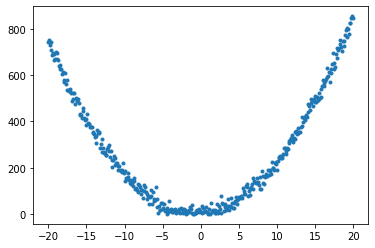
\includegraphics[scale=.35]{img/explicaciones/1_seg.png}
            \caption{Gráfico del conjunto de datos}
        \end{subfigure}
        \begin{subfigure}{.3\textwidth}
            \centering
            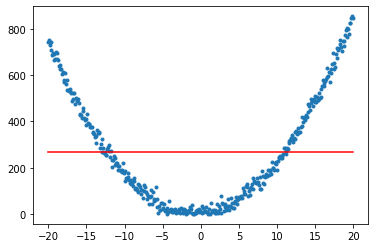
\includegraphics[scale=.35]{img/explicaciones/2_seg.png}
            \caption{Regresor, sin segmentar}
        \end{subfigure}
        \begin{subfigure}{.3\textwidth}
            \centering
            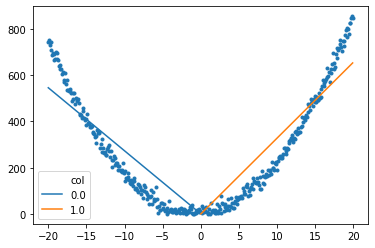
\includegraphics[scale=.35]{img/explicaciones/3_seg.png}
            \caption{Regresor, segmentando}
        \end{subfigure}
        \caption{Ejemplos de modelos con y sin segmentación}
        \label{segs}
    \end{figure}
        
        %Cuando se desea hacer una regresión, se tiene un conjunto de datos, llamadas muestras, los cuales tienen variables independientes involucradas.
        
        %Estas variables, para el caso particular que tratamos, son los \textit{metros cubiertos}, \textit{la cantidad de baños}, etc. Estas variables son numéricas, y reflejan una cantidad de algo.
        
        %Pero por el otro lado, también se tienen la \textit{ciudad}, la \textit{provincia}, etc. A diferencia de las anteriores, estas son variables \textit{categóricas}, y 2 valores distintos de alguna de ellas no tiene ninguna relación.
        
        %Si bien solo se pueden utilizar variables numéricas de manera directa para los regresores explicados hasta ahora, hay una forma distinta de construir un regresor, utilizando la técnica de segmentación.
        
        %La segmentación busca separar las muestras en base a los valores de una variable independiente, ya sea numérica o categórica. Luego, al tener las muestras divididas en grupos, se aplica el \textit{fitting} a cada grupo, obteniendo así un regresor por cada valor de la variable independiente utilizada para segmentar. Aplicando esta técnica a un regresor lineal por ejemplo, se obtiene lo que se llama un regresor lineal segmentado, el cual se muestra a continuación:
    
        Esta técnica tiene como objetivo poder establecer una mejor relación entre la variable a describir y las utilizadas para describirla. En este caso, se puede observar que, segmentar según el signo de la variable $x$, resulta ser beneficioso. Una aclaración que vale la pena mencionar, es que, aunque nos estemos refiriendo a la misma variable $x$, podría pensarse como que la misma se dividió en dos, la variable $x_{<0}$, que se tiene en consideración para un modelo, y la variable $x_{>0}$, que se tiene en consideración en el otro.

        Es importante notar que, no siempre será beneficioso aplicar segmentación sobre los datos. Por ejemplo, si las muestras resultantes luego de segmentar no poseen una cantidad de datos significativa, esto puede causar un \emph{overfitting}. Esto se debe a que, cuando las relaciones subyacentes no están bien definidas, segmentar no aporta un beneficio, y la conclusión es que estamos entrenando nuestros modelos con menos datos.

\subsection{Fitting}
    
    Luego de definirse un modelo para regresión, nos interesa encontrar el valor óptimo de $\beta$, es decir, de los parámetros desconocidos, tal que el error de la predicción es el mínimo posible. Para esto, primero definimos la ecuación que involucra a cada $Y_i$ con los $X_i$ y las $f_j$ en forma matricial, aprovechando que es una combinación lineal de funciones:
    
    \begin{equation}
\begin{bmatrix}
 Y_1 \\ \vdots \\ Y_{n} 
 \end{bmatrix}
 =
 \begin{pmatrix}
  f_1(X_{11}) && \ldots & f_k(X_{1k}) \\
  \vdots && \ddots & \vdots \\
  f_1(X_{n1}) && \ldots & f_k(X_{nk})
  \end{pmatrix}
  \times
  \begin{pmatrix}
  \beta_1 \\ \vdots \\ \beta_k
  \end{pmatrix}
  +
  \begin{pmatrix}
  e_1 \\ \vdots \\ e_k
  \end{pmatrix}
\end{equation}
    
    Luego, nos interesa minimizar cada $e_i$, que es equivalente a minimizar la norma del vector $e$. Luego, si dejamos el error en función de las demás variables, tenemos este sistema:
    
    \[ b - Ax = e  \implies ||b - Ax||_2 = ||e||_2 \]
    
    Donde b es el vector Y, A es la matriz anterior con elementos $f_i(X_{ji})$, $x$ es el vector $\beta$ a determinar, y $e$ es el vector de los errores individuales. Como queremos minimizar la norma de $e$, podemos plantear este sistema y obtendremos el x ($\beta$) que minimiza el $e$ (error):
    
    \[ \min_x  ||b - Ax||_2\]
    
    Transformando el problema de encontrar el $\beta$ óptimo a esto, podemos aplicar un método conocido para resolver esto.
    
    \subsubsection{CML (Cuadrados Mínimos Lineales)}
    
    Cuadrados mínimos lineales es un método utilizado para encontrar el $x$ que minimiza esa norma de manera directa. Para esto, utiliza lo que se llama \textit{Ecuaciones Normales} que transforma el problema en uno equivalente, basado en la resolución de un sistema lineal:
    
    \[ \min_x  ||b - Ax||_2 \iff A^T A x = A^T b\]
    
    Al método se le atribuye este nombre porque busca minimizar la norma, que termina siendo equivalente a minimizar la suma de cuadrados, que son las diferencias entre cada estimación y su valor real al cuadrado. Entonces, se obtiene un valor para el vector $x$, es decir nuestro $\beta$, que minimiza esta suma de cuadrados, que visto para el caso de regresión lineal gráficamente se ve así:
    
    \begin{figure}[H]
        \begin{center}
            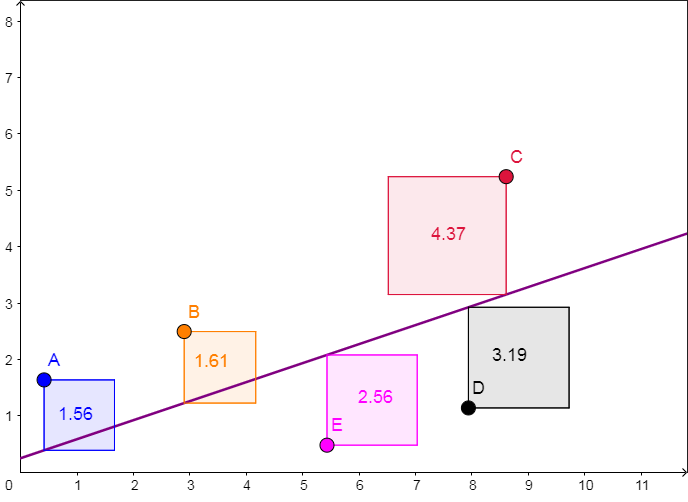
\includegraphics[scale=0.4]{img/explicaciones/CML-Line.png}
            \end{center}
    \end{figure}
    
    Donde la recta es la que minimiza las áreas de esos cuadrados, que surgen de hacer las diferencia entre lo que estimó la recta y el valor real, es decir, cada punto que aparece ahí.
   

\subsection{Feature engineering}

Generalmente, el conjunto de datos a estudiar contiene más información de la que puede utilizar un modelo, entre estos datos se encuentran variables categóricas, o numéricas que, por si solas, no aportan información estadísticamente relevante. Por estos motivos, existe una técnica llamada \fe, que busca reutilizar esta información, combinándola de diversas maneras (ponderándolas, aplicándoles operadores lógicos, etc.), y así derivar una nueva característica que sí exhiba una relación relevante. Estas nuevas características pueden ser utilizadas para segmentar el conjunto de datos, con la finalidad de aumentar la precisión del modelo.



\subsection{Evaluación de modelo}  
    Luego de construir un modelo, es importante poder determinar qué tan bueno es para predecir la variable dependiente. La manera de hacer esto es, después de entrenar nuestro modelo, comparar los resultados obtenidos con los datos reales.
    
    %decir que tan bueno es, se debe observar su capacidad de estimar la variable dependiente ( la que se quiere predecir ) en base a valores de las variables independientes ( predictores ) y comparar el error de la estimación con respecto al valor real de la variable dependiente.
    
    \subsubsection{Métricas}
  
    Para realizar estas comparaciones, una primera idea suele ser medir el promedio de las diferencias absolutas entre los datos reales, y nuestras predicciones. El problema con esta idea es que hay casos donde esta métrica puede verse afectada según la naturaleza de la variable que se intenta predecir. En pos de solucionar los problemas que pueda tener una métrica en particular, lo que se hace es tener en cuenta un conjunto de ellas, con la intención de obtener los modelos con los mejores resultados en conjunto. A continuación, exponemos las métricas que usamos en nuestra experimentación.
    
    %Para poder llevar a cabo esta comparación, hay varias métricas que la resuelven, de las cuales mencionamos las tres que consideramos para nuestro análisis.

        \paragraph{RMSE (Root Mean Squared Error)}\mbox{}\vspace{1em}
        
        Una métrica un poco más avanzada que el promedio de las diferencias absolutas, y en sintonía con el método de cuadrados mínimos, es la que se conoce como \emph{RMSE} (root mean squared error), que consiste en calcular la raíz cuadrada del promedio de los errores cuadráticos entre las predicciones y los datos. Formalmente, la métrica está definida de la siguiente manera:
        %Una primera idea para calcular el error cometido en la predicción es la del RMSE ( Root Mean Squared Error ), que equivale a hacer:
        
        \[ RMSE= \sqrt{\frac{1}{n}\sum_{j=1}^{n} (f(X_j) - Y_j)^2}\]
        
        Donde $X_j$ la muestra $j$-esima, $f$ es la función del modelo, y $Y_j$ es el valor real a predecir para cada muestra.
        
        Esta métrica busca representar al error cometido al estimar como el promedio de los errores cometidos para cada valor de la variable dependiente $y$. Esta métrica resulta intuitiva y razonable, porque es  lo que se puede pensar en hacer en una primera instancia, pero presenta un problema grave.
        
        %Esta métrica busca , a grandes rasgos, representar al error cometido al estimar como el promedio de los errores cometidos para cada valor de la variable dependiente $y$. Esta métrica resulta intuitiva y razonable, porque es lo que se puede pensar en hacer en una primera instancia, pero presenta un problema grave.
        
        El defecto del \emph{RMSE} es que, cuando se comete un error grande para cierto valor de $y$, eso repercute mucho en el promedio de los errores. Es decir, si había un valor a estimar que era grande comparado con otros valores que tomaba la variable $y$, este va a tener mayor peso en el error que otros.
        
        \paragraph{RMSLE (Root Mean Logarithm Squared Error)}\mbox{}\vspace{1em}
        
        Existe una segunda métrica casi idéntica a la anterior, que introduce al calculo de \emph{RMSE} una solución al problema que tiene el mismo. Podemos ver a continuación la nueva definición del error:
        
        \[ RMSLE= \sqrt{\frac{1}{n}\sum_{j=1}^{n} (\log{(f(X_j))} - \log{(Y_j)})^2}\]
        
        Donde $X_j$, $f$ e $Y_j$ son las mismas que en \emph{RMSE}.
        
        Lo que cambia en este caso, es que ahora no se calcula la diferencia directamente, sino que primero se aplica el logaritmo a ambos términos, tanto $f(x)$ como $y$, antes de realizar la diferencia entre ellos.
        
        La idea atrás de esto es que, si bien RMSE tiene sentido, tiene problemas al tratar con variables que presentan valores grandes, como son los outliers. Entonces, como solución, se le aplica el logaritmo a estas variables, para luego poder trabajar con números mas pequeños, y que todos aporten equitativamente al calculo del error.
        
        
        \paragraph{$\mathbf{R^2}$ (R-squared)}\mbox{}\vspace{1em}
        
        Además de interesarnos por medir el error de un modelo, nos interesó también poder capturar si había espacio para mejorarlo. Para poder analizar esto, optamos por utilizar la métrica R2, la cual se muestra a continuación:
        
        \[ R2= 1 - \frac{\sum_{j=1}^{n} (f(X_j) - Y_j)^2}
                    {\sum_{j=1}^{n} (\overline{Y} - Y_j)^2}\]
        
        Donde $X_j$, $f$ e $Y_j$ son las mismas que en $RMSE$, y $\overline{Y}$ es la media de las muestras $Y_j$.
        
        Es importante notar que el resultado suele variar entre 0 y 1 , siendo 1 el resultado de un modelo que no puede mejorase, y por lo contrario, 0 el resultado si hubiéramos tomado el promedio. Sin embargo, en la práctica podría suceder que un modelo sea peor que el promedio, lo cual llevaría a un r2 negativo. Lo que refleja este calculo se puede ver mejor en este gráfico:
        
        \begin{figure}[H]
            \centering
            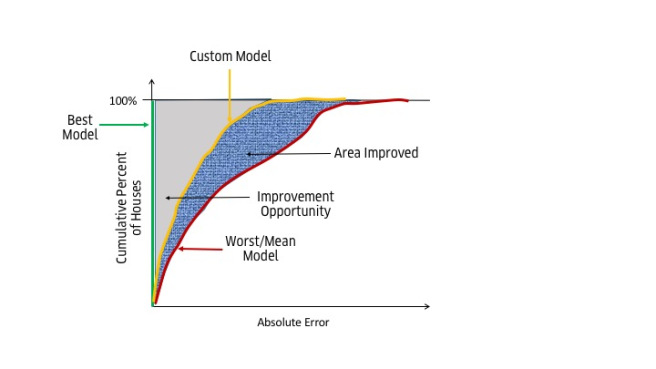
\includegraphics[scale=0.5]{img/explicaciones/R2-Curves.jpg}
            \caption{Resultado del \textit{Curvas de R2}}
            \label{fig:R2-Curves}
        \end{figure}
        
        En este se muestran 3 curvas, una por cada posible modelo.
        El \textbf{Best Model} es el mejor modelo teórico, donde el error acumulado siempre es 0. Luego se tiene el \textbf{Worst Model}, que representa a un regresor que solo tiene en cuenta el promedio de los datos.
        Finalmente, se tiene al \textbf{Custom Model}, el modelo que uno diseña, el cual tiene un error que se encuentra entre la del mejor y el peor modelo. También se puede observar que la manera de interpretar el gráfico es observando el área debajo de la curva de un modelo.
        Si observamos la curva del \textbf{Custom Model}, observamos que el área azul encerrada entre esta curva y la del \textbf{Worst Model} indica cuanto se mejoró con respecto a este último. Así también, el área gris, encerrada entre el \textbf{Custom Model} y el \textbf{Best Model}, indica cuanto puede mejorarse para parecerse a este ultimo modelo.
        
\subsubsection{K-Fold cross validation}

 %   determinar como se generalizan estos resultados en práctica. Teniendo simplemente dos conjuntos de datos, uno de entrenamiento, y otro de preba, a veces el modelo es suceptible a la distribución de los datos de entrenamiento. El objetivo del método de \cv es intentar aisalar al modelo, de problemas como  \emph{overfitting} o \emph{selection bias}, y mostrar como operaria el modelo con datos independiente. K fold cross validarion es dividir el dataset en $k$ particiones de igual tamaño.
    
    Al utilizar estas métricas para medir el error o la mejora de un modelo, se suele definir un conjunto de training y otro de validation. Luego, se hace un \textit{training} del modelo con el primer conjunto, y luego se aplica el \textit{predict} sobre el segundo conjunto. Y finalmente, se aplica alguna de las métricas sobre el resultado del \textit{predict}, y se obtiene el error cometido o si se mejoró o no el modelo.
    
    El problema de este procedimiento es que se esta definiendo un conjunto como training y otro como validation, y no se los cambia más. Esto provoca que al minimizar, por ejemplo, el error, bajo un mismo conjunto no necesariamente implica que en el caso general sea mejor, ya que no se está midiendo para distintos conjuntos de training y validation.
    
    Una forma de solucionar este problema es la de intentar evaluar bajo distintos conjuntos de training y validation y tomar el promedio de todos ellos. Para esto existe la técnica de \emph{K-Fold cross validation}, que busca solucionar el problema mencionado aplicando variaciones en los conjuntos para luego aplicar las métricas. Podemos ver esto mas claramente en el siguiente diagrama:
    
    \begin{figure}[H]
        \begin{center}
            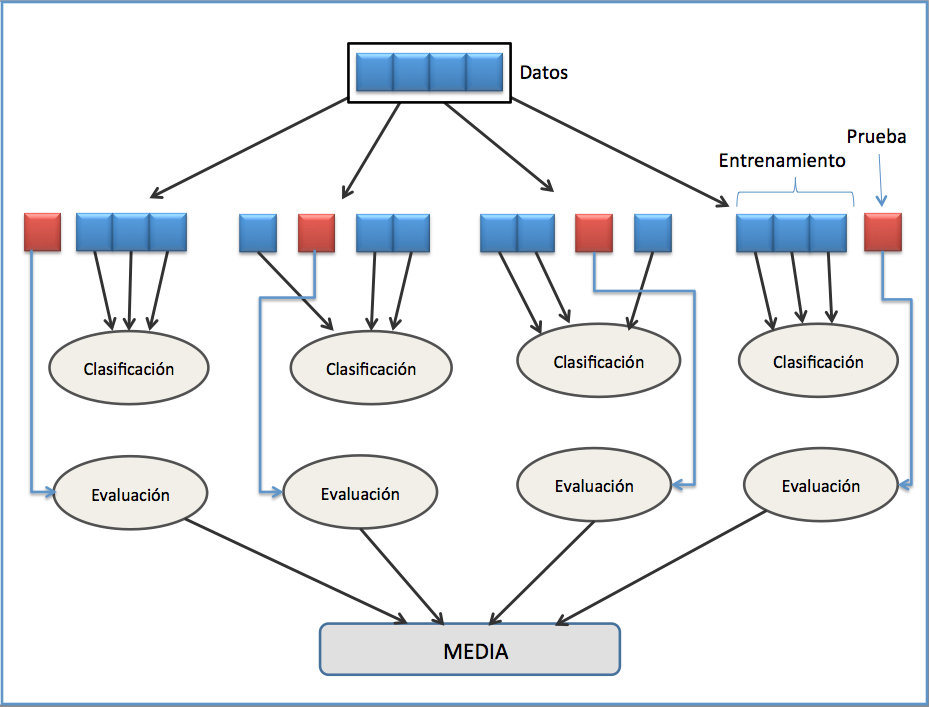
\includegraphics[scale=0.3]{img/explicaciones/k_fold.png}
        \end{center}
        \caption{Diagrama K-Fold}
    \end{figure}
    
    En este caso particular, se tiene un conjunto de datos que se lo divide en 4 conjuntos de igual tamaño. Luego, se toma en cada caso 3 conjuntos para training y el otro para validation. Con estos 2 nuevos conjuntos finales de training y de validation, se entrena al modelo y luego se lo evalúa, generando un resultado. Este proceso se repite para cada variación de conjunto de training y validation, y se obtiene la media de los resultados obtenidos. Esta media va a ser entonces la que se va a intentar maximizar bajo el criterio establecido.

\subsection{Feature selection}
    Una primera idea a la hora de elegir los features de nuestro modelo, es considerar todas las combinaciones posibles de elementos del conjunto de features. Es decir, si el conjunto de features tiene $p$ elementos, consideramos los $p$ modelos con un único feature, luego, consideramos los $\binom{p}{2}$ modelos con dos predictores, y así sucesivamente. El problema con este método es que, la cantidad de modelos a comparar aumenta exponencialmente con el número de features, exactamente, si $p$ es el número de features, entonces  la cantidad de modelos a comparar es $\sum_{k=0}^{p}\binom{p}{k} = 2^p$. Un método menos exacto pero más conservador con respecto a la cantidad de modelos a comparar es el que se conoce como \fss, que pasaremos a explicar a continuación.

\subsubsection{Forward stepwise selection}
    Como mencionamos antes, quisiéramos una manera de seleccionar un modelo, relativamente competente, sin necesidad de clasificar todo el universo de modelos con hasta $p$ features, que como vimos anteriormente, consiste de $2^p$ elementos. La idea de este método es obtener modelos de forma iterativa, y en particular agregativa. El método consiste en ir agregando features, de a una por vez, a un modelo anterior, y eligiendo aquella que mayor impacto tenga en el rendimiento del modelo, este proceso se repite, considerando este nuevo modelo, como el modelo anterior a agregarse features. Formalmente, el método esta definido por el siguiente algoritmo \cite{islr}.
    
    
    \begin{algorithm}[H]
    \begin{enumerate}
        \item Sea $\mathcal{M}_0$ el modelo sin predictores.
        \item Para $k=0, \dots ,p-1$:
        \begin{enumerate}
            \item Consideremos todos los $p-k$ modelos que añaden un predictor al modelo $\mathcal{M}_k$.
            \item Elegimos el \emph{mejor} de estos $p-k$ modelos, y lo llamamos $\mathcal{M}_{k+1}$. Donde \emph{mejor} está definido como el modelo con mayor precisión respecto a la métrica $R^2$.
        \end{enumerate}
        \item Elegimos el mejor modelo del conjunto de los $\mathcal{M}_0,\dots,\mathcal{M}_p$ usando \cv, con respecto a la métrica $R^2$.
    \end{enumerate}
         \caption{Forward stepwise selection}
    \end{algorithm}

    %\begin{enumerate}
    %    \item Sea $\mathcal{M}_0$ el modelo sin predictores.
    %    \item Para $k=0, \dots ,p-1$:
    %    \begin{enumerate}
    %        \item Consideremos todos los $p-k$ modelos que añaden un predictor %al modelo $\mathcal{M}_k$.
    %        \item Elegimos el \emph{mejor} de estos $p-k$ modelos, y lo llamamos $\mathcal{M}_{k+1}$. Donde \emph{mejor} está definido como el modelo con mayor precisión respecto a la métrica $R^2$.
    %    \end{enumerate}
    %    \item Elegimos el mejor modelo del conjunto de los $\mathcal{M}_0,\dots,\mathcal{M}_p$ usando \emph{cross validation}, con respecto a la métrica $R^2$.
    %\end{enumerate}
    
    No obstante, no es cierto que este método siempre encuentre el mejor modelo posible dadas las features que tenemos a nuestra disposición. Por ejemplo, supongamos un conjunto de muestras que poseen $p = 3$ predictores. Puede suceder que el mejor modelo con una única variable, sea aquel que contiene al predictor $X_1$, mientras que el mejor modelo posible sea aquel que contiene a los predictores $X_2$ y $X_3$. Entonces, el método no podrá obtener el mejor modelo posible ya que, todos los modelos en la selección final del método, tendrán que contener a $X_1$. Esta es la concesión que hacemos al usar este método, a cambio reducimos las comparaciones a realizar a $\sum_{i=1}^{p}i = \frac{p(p+1)}{2}.$
    
\subsubsection{Matriz de correlación}
    
    Cuando se deben elegir las variables o features que se utilizaran en el modelo, se puede optar por distintos criterios. Un criterio es el de observar individualmente a través de un gráfico, la relación entre la variable a predecir y la que se utilizará para describirla. Si bien esto suena razonable, optamos también por observar otro aspecto, las correlaciones entre ellas. 
    
    La correlación entre dos variables $X$ e $Y$ nos indica la dependencia entre ellas, es decir, si existe una relación. El valor de la correlación entre ellas esta acotado entre -1 y 1, donde:
    
    \begin{itemize}
        \item Si el valor es cercano a 1 indica que tienen una relación lineal (correlación), cuando $X$ cambia, $Y$ se incrementa linealmente.
        
        \item Si el valor es cercano a -1 indica que tienen una relación lineal inversa (anticorrelación), cuando $X$ cambia, $Y$ decrementa linealmente.
        
        \item Si el valor es cercano a 0 indica que no hay mucha relación (incorrelación).
        
        \item Si el valor esta en el medio de los anteriores, indica el nivel de relación lineal que hay entre las variables.
    \end{itemize}
    
    Bajo este criterio, podemos decir que, dada una variable que queramos predecir, podemos observar sus correlaciones con las demás, y con eso deducir cuales serán mejores para describirla. Esto se puede analizar mediante una matriz de correlación, como la que se muestra a continuación:
    
    \begin{figure}[H]
        \begin{center}
            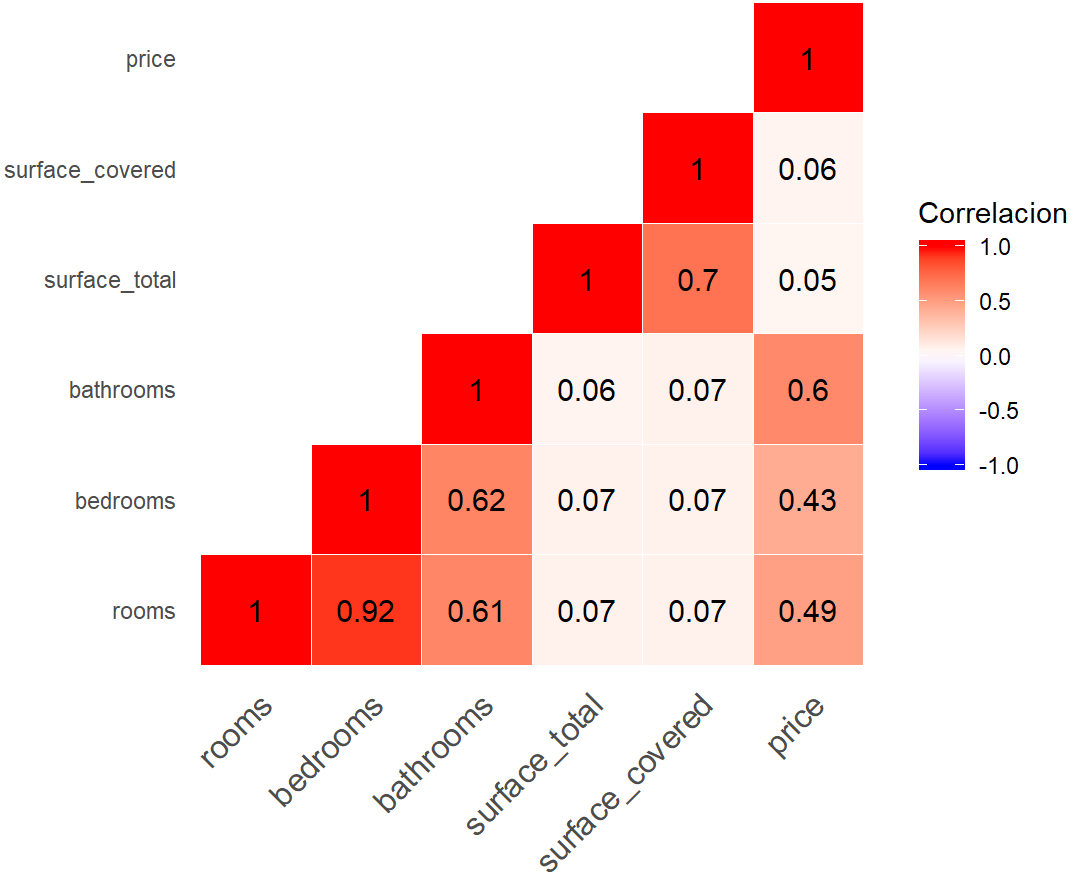
\includegraphics[scale=0.6]{img/explicaciones/Corr-Matrix-Heatmap.png}
            \caption{Matriz de correlación entre características de casas}
            \end{center}
    \end{figure}
    
    En la matriz de la figura anterior, podemos ver la relación de precio con las demás variables. Tenemos por ejemplo, que precio tiene una correlación de 0.49 con habitaciones, 0.43 con dormitorios, y de 0.6 con baños. Esto nos indica que parece buena idea intentar explicar precio con estas 3 variables, sin embargo para metros totales y cubiertos, se tiene 0.05 y 0.06 respectivamente, cercano a 0. Esto ultimo nos indica que no parecen tener relación alguna, y por lo tanto, se puede sospechar que no sean útiles para explicarlo.
    
    Otro punto interesante que nos provee la matriz de correlación, es la relación que hay entre las variables que se quieren utilizar para predecir. Cuando se tienen 2 variables en un modelo que presentan una correlación alta, nos indica que una puede utilizarse para describir a la otra, entonces incluir ambas en el modelo, agregaría redundancia. Por el otro lado, si estas cerca de estar incorrelacionadas, significa que cada una termina aportando información extra a la hora de describir. En el caso del ejemplo anterior, podemos ver que la relación entre dormitorios y habitaciones es de 0.92, lo cual indica que están fuertemente correlacionadas, y es seguro pensar que descartar una de las dos para el modelo final será mejor.
    
    




\section{Construcción de los modelos}

    \subsection{Feature Engineering}
    \subsubsection{Chetocidad}
    
    Viendo las columnas presentes en \emph{dataset}, nos llamaron la atención varias características, que, cuando presentes en un inmueble, normalmente uno asociaría con un alto precio. Deseamos capturar esta relación haciendo uso de la técnica de \fe. Naturalmente, decidimos llamar a esta feature \textbf{chetocidad}. La definimos de la siguiente manera para cada \emph{entry}:

        $$chetocidad = gimnasio + piscina + usosmultiple + garages.$$
    
    Haremos uso de ella para segmentar el conjunto de datos, y poder predecir mejor el precio en cada uno.

    \begin{figure}[H]
        \centering
        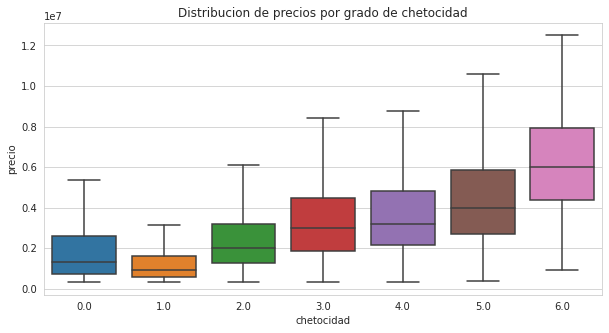
\includegraphics[scale=0.7]{img/cmp/precio/dist-chetocidad.png}
        \caption{}
        \label{fig:precio-dist-chetocidad}
    \end{figure}
    
    En la figura (\ref{fig:precio-dist-chetocidad}) se puede ver como a medida que el \emph{grado} de chetocidad incrementa, también lo hacen los precios.
    
    \subsubsection{WordCloud}
    
    Dos características interesantes presentes en el conjunto de datos son el \textbf{título} y la \textbf{descripción}. La intuición que tenemos es que, para inmuebles donde se parezcan estas dos, podrían llegar a tener características similares, por ejemplo el precio. Explicaremos nuestro procedimiento para el título, ya que para la descripción es un proceso análogo.
    
    Buscamos asignarle a cada inmueble un \emph{score} calculado a partir de su titulo. Para ello, la forma más simple que se nos ocurrió comienza con tomar todos los títulos de todos los inmuebles, y ver la cantidad de ocurrencias que tiene cada palabra del vocabulario que elijamos.
    
    Por ejemplo, si tuviéramos 3 propiedades, con títulos:
    
    \begin{verbatim}
        inmueble    titulo
        1           casa en venta
        2           casa en venta
        3           casa en venta en tijuana
    \end{verbatim}

    Omitiendo palabras como conectores ya que no aportan a lo que buscamos, nos quedarían las siguientes apariciones para cada palabra:
    
    \begin{verbatim}
        word        #
        casa        3
        venta       3
        tijuana     1
    \end{verbatim}
    
    Finalmente, para computar los \emph{scores} de cada titulo, tomamos el promedio de las apariciones de cada una de sus palabras. Esto nos da lo que llamamos \textit{frecuencia promedio de apariciones}, o, abreviado, \textit{avg\_freq\_title}:
    
    \begin{verbatim}
        inmueble    titulo                          avg_freq_title
        1           casa en venta                   (3 + 3) / 2 = 3
        2           casa en venta                   (3 + 3) / 2 = 3
        3           casa en tijuana                 (3 + 1) / 2 = 2
    \end{verbatim}
    
    De esta forma, logramos asignarle a cada inmueble un puntaje basado en su titulo.
    Nuestra hipótesis entonces es que resulta una característica sensata, que podría dar buenos resultados, pero tiene una fuerte dependencia en la naturaleza de los datos. Por su heterogeneidad, podría suceder que no necesariamente haya una relación entre inmuebles con títulos similares, a pesar de que sea intuitivo pensar que sí.
    
    \begin{figure}[H]
        \begin{subfigure}{.49\textwidth}
            \centering
            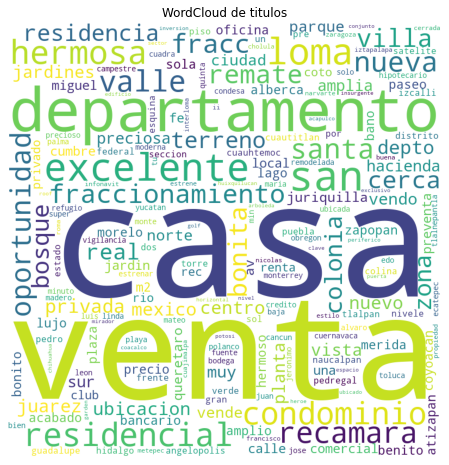
\includegraphics[scale=.5]{img/cmp/wc/wc-title.png}
            \caption{Títulos}
        \end{subfigure}
        \begin{subfigure}{.49\textwidth}
            \centering
            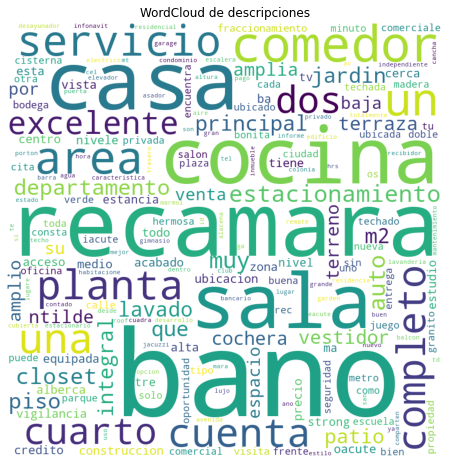
\includegraphics[scale=.5]{img/cmp/wc/wc-desc.png}
            \caption{Descripciones}
        \end{subfigure}
        \caption{WordClouds de campos de texto}
        \label{fig:wc}
    \end{figure}
    
    En la figura (\ref{fig:wc}), se puede observar como están distribuidas las distintas palabras que componen los campos de texto a considerar. Veamos las frecuencias obtenidas. 
    
    \begin{figure}[H]
        \centering
        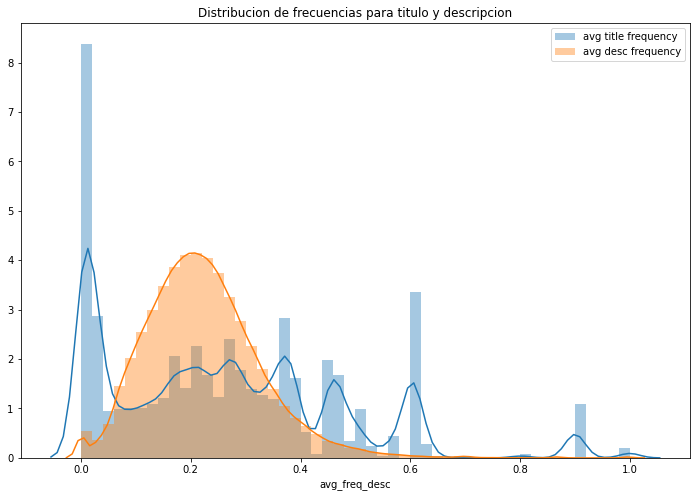
\includegraphics[scale=0.6]{img/cmp/wc/freq.png}
        \caption{Distribución de frecuencias}
        \label{fig:wc-freq}
    \end{figure}
    
    Y finalmente en (\ref{fig:wc-freq}) graficamos la distribución de los scores resultantes, que además normalizamos de 0 a 1 por min-max para simplificar.
    
    \subsection{Segmentación}
    
    Las variables categóricas que elegimos para segmentar el conjunto de datos son diferentes para cada variable a predecir, pero siempre incluimos la opción de \textbf{no} segmentar, para tenerla como base. 
    
    Para fortalecer nuestras intuiciones, graficamos en algunos casos a modo de ejemplo la distribución que tienen los datos segmentando por las variables a considerar. Que sean conjuntos que varían mucho entre sí, incluso disjuntos, nos llevaría a pensar que puede valer la pena entrenar a los clasificadores por separado.
    
    \subsubsection{Precio}
    
    Consideramos,
    
    \begin{itemize}
        \item \textbf{Provincia}: Es a la que le tenemos más expectativa. Como se puede ver en \ref{fig:precio-dist-provincia}, está bien marcada la diferencia entre las distribuciones de los precios para cada ciudad, y luego consideramos que verlas por separado evitará ruido, logrando que expliquemos mejor el precio.
        
            \begin{figure}[H]
                \centering
                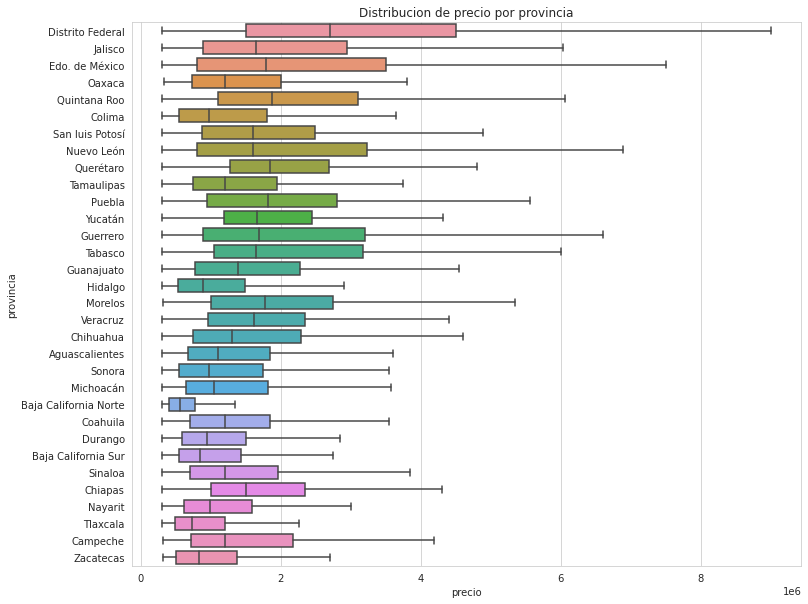
\includegraphics[scale=0.45]{img/cmp/precio/dist-provincia.png}
                \caption{Distribución por provincia}
                \label{fig:precio-dist-provincia}
            \end{figure}
        
        \item \textbf{Ciudad}: Diferentes ciudades tendrán diferentes situaciones económicas, y diferentes tipos de inmuebles con diferentes precios. Como son muchas (~800) podría llegar a generar un problema ya que los conjuntos de datos resultantes serán muy pequeños.
        \item \textbf{Chetocidad}: Como ya fue discutido en la figura \ref{fig:precio-dist-chetocidad}, inmuebles mas chetos tienden a ser mas caros.
        \item \textbf{Antiguedad}: Los inmuebles mas antiguos tienden a ser más caros.
    \end{itemize}
    
    \subsubsection{Metros cubiertos}
    
    Consideramos las siguientes,
    
    \begin{itemize}
        \item \textbf{Tipo de propiedad}: Intuitivamente, cada tipo de propiedad tendrá un cantidad de metros cubiertos que varíe. Nuestra hipótesis es que esta será la mejor.
        
        \begin{figure}[H]
            \centering
            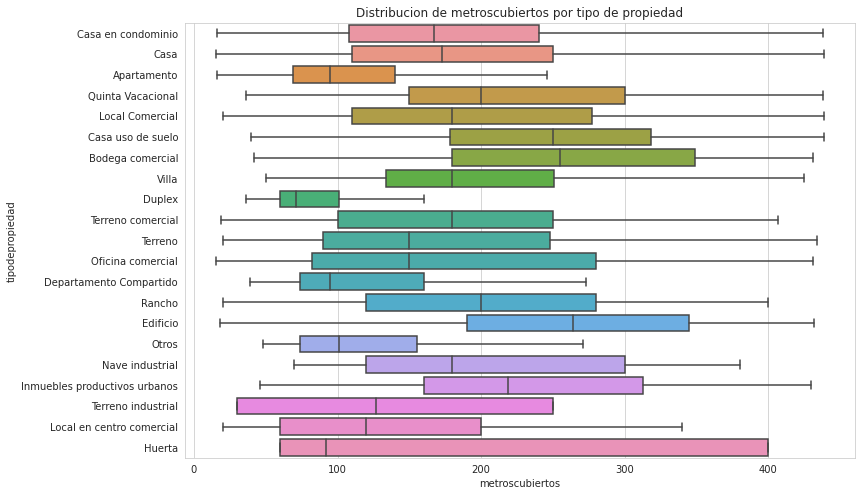
\includegraphics[scale=0.45]{img/cmp/metroscubiertos/dist-tipodepropiedad.png}
            \caption{Distribución por tipo de propiedad}
            \label{fig:m2-dist-prop}
        \end{figure}
        
        \item \textbf{Antiguedad}: Las casas más antiguas suelen ser más grandes, mientras que las más nuevas más chicas. Como se puede ver en \ref{fig:m2-dist-ant}, no es tan pronunciada como esperábamos.
        
        \begin{figure}[H]
            \centering
            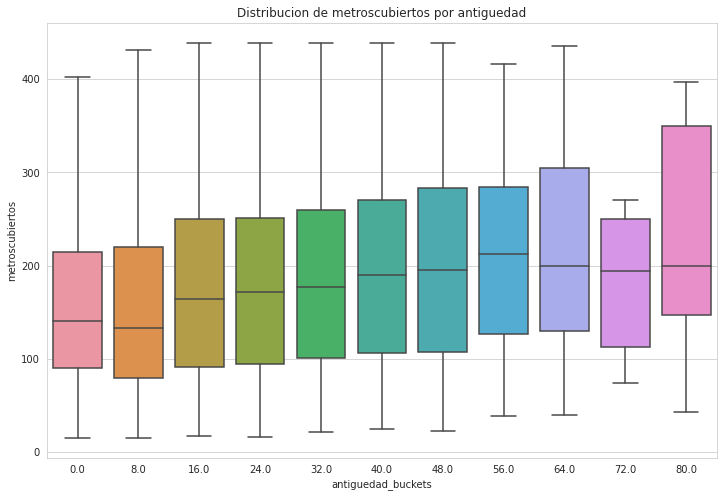
\includegraphics[scale=0.45]{img/cmp/metroscubiertos/dist-antiguedad.png}
            \caption{Distribución por antiguedad}
            \label{fig:m2-dist-ant}
        \end{figure}

        \item \textbf{Chetocidad}: A pesar de que este feature fue introducido originalmente para precios, las casas mas chetas suelen ser más grandes. Pero en la figura \ref{fig:m2-dist-chet} se observa como esta relación no es tan pronunciada como en el caso de la variable precio.
        
        \begin{figure}[H]
            \centering
            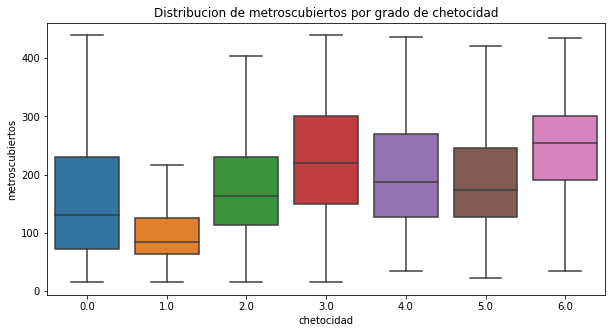
\includegraphics[scale=0.45]{img/cmp/metroscubiertos/dist-chetocidad.png}
            \caption{Distribución por chetocidad}
            \label{fig:m2-dist-chet}
        \end{figure}
    \end{itemize}
    
    \subsubsection{Segmentar o no segmentar, esa es la cuestión}
    
    Como discutimos anteriormente, al segmentar, un riesgo que corremos es que los conjuntos de datos resultantes sean demasiado pequeños, lo que llevaría a que el clasificador resultante esté potencialmente \textit{overfitteado} a esos datos. Por ejemplo, al haber tantas ciudades, es posible que esto suceda al segmentar por ellas.

    \subsection{Selección de features}
    
    Una vez definidas las categorías por las cuáles queríamos segmentar, necesitábamos alguna manera de determinar, qué features debía incluir finalmente nuestro modelo. Entonces, un primer paso era, basados en los resultados de la matriz de correlación (Figura \ref{corr}), filtrar los features mas útiles a considerar para la selección en el segundo paso. Este primer paso se puede observar a continuación:
    \begin{figure}[H]
        \centering
        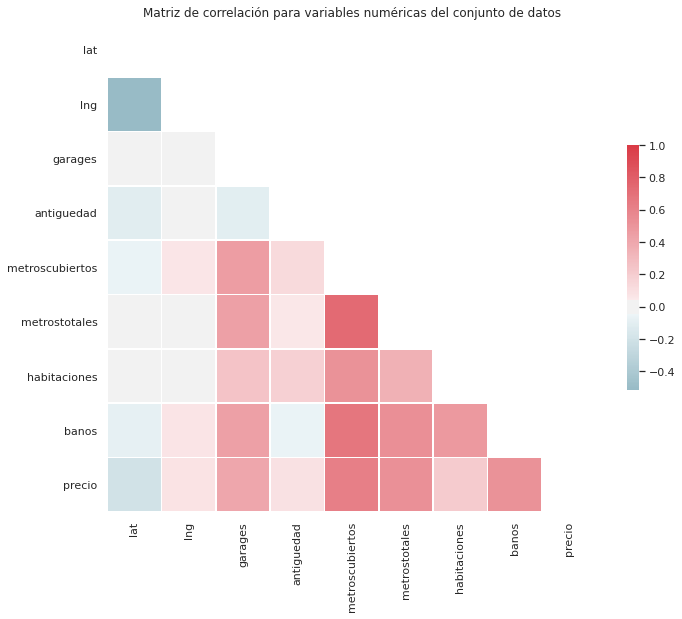
\includegraphics[scale=0.5]{img/cmp/1_corr.png}
        \caption{Matriz de correlación}
        \label{corr}
    \end{figure}
    
    Considerando solo las variables con un índice de correlación mayor a 0.2 con precio en esta matriz, obtuvimos el conjunto inicial de features compuesto por:
    

        \begin{verbatim}
            features = [
                    'metroscubiertos',
                    'antiguedad',
                    'banos',
                    'garages',
                    'metrostotales',
                    'habitaciones'
            ]
        \end{verbatim}
    
    Luego, el segundo paso consistió en utilizar el método \fss \ que se explicó en secciones anteriores, para seleccionar los features finales para cada modelo basándonos en los obtenidos en el paso 1. En este paso tuvimos en cuenta distintos tipos de modelos, entre ellos, regresores lineales, polinomiales y de proyección. Los resultados para distintas selecciones de features para cada modelo se observan en la figura (\ref{fss}):
     
    \begin{figure}[H]
        \centering
        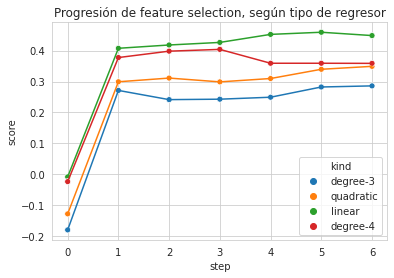
\includegraphics[scale=0.6]{img/cmp/1_fss.png}
        \caption{Progresión del score (que equivale a R2) para distintos modelos a medida que se sumaban variables a cada uno.}
        \label{fss}
    \end{figure}
    Consideramos que la mejor selección de features para cada modelo en en este caso era la que maximizaba el score.
    
    \subsection{Clasificadores a considerar}
    
    Los clasificadores que comparamos se muestran a continuación, donde cada uno se combino con cada posible segmentación descripta anteriormente. Para cada uno definimos un \textit{kind}, que podía ser polinomial o de proyección, y una lista de features a considerar, las cuales pueden haber sido escogidas por pura intuición o mediante un mecanismo automático como \fss.
    
    \paragraph{Precio}\mbox{}\vspace{1em}
    
    Incluimos como control el regresor más simple: explicar precio a través de metroscubiertos con una proyección.
    
    \begin{figure}[H]
    \centering
    \begin{tabular}{ |c|c|c| } 
    \hline
    kind                    & feature       & elección \\ \hline
    projection              & metroscubiertos & control \\ \hline
    projection con freqs    & metroscubiertos, avg\_freq\_title, avg\_freq\_desc & a ojo \\ \hline
    quadratic               & metroscubiertos, metrostotales & forward stepwise \\ \hline
    linear                  & metroscubiertos, metrostotales, banos, habitaciones & forward stepwise \\ \hline
    degree 4                & metroscubiertos, metrostotales, habitaciones & forward stepwise \\ \hline
    \end{tabular}
    \caption{Features por cada clasificador}
    \end{figure}
    
    \subsection{Metroscubiertos}
    
    Las features en este caso fueron elegidas a ojo, y las que consideramos que mejor podían explicar los metros cubiertos de un inmueble son las \textit{habitaciones}
    , \textit{cantidad de baños} y finalmente \textit{precio}. Los tipos a considerar son \textit{linear}, \textit{quadratic} y \textit{projection}.

\section{Discusión de los resultados}

A continuación procedemos a presentar los resultados obtenidos para cada clasificador. Consideramos las métricas de scoring \textit{r2}, \textit{rmse} y \textit{rmsle}. Y ordenamos los resultados por \textit{r2}.

\subsection{Precio}

\begin{figure}[H]
\centering
\begin{tabular}{ |c|c|c|c|c|c| } 
\hline
\textbf{rank} & kind & segment\_by & r2 & rmse & rmsle \\ \hline
0 & linear & provincia & 0.5419 & 1191109.9895 & 0.5043 \\ \hline
1 & linear & None & 0.4512 & 1307140.9522 & 0.5536 \\ \hline
2 & degree 4 & None & 0.4285 & 1431781.8520 & 0.5671 \\ \hline
3 & projection con freqs & antiguedad & 0.4191 & 1563665.8240 & 0.5833 \\ \hline
4 & projection & antiguedad & 0.4187 & 1564135.4745 & 0.5764 \\ \hline
5 & quadratic & None & 0.4137 & 1456341.1900 & 0.5747 \\ \hline
6 & projection con freqs & None & 0.4009 & 1600473.7443 & 0.5850 \\ \hline
7 & projection & None & 0.3941 & 1609558.2153 & 0.5928 \\ \hline
8 & degree 4 & chetocidad & 0.3921 & 1392346.0420 & 0.5670 \\ \hline
9 & degree 4 & provincia & 0.3892 & 1463775.4949 & 0.5861 \\ \hline
10 & linear & antiguedad & 0.3811 & 1374499.6945 & 0.5946 \\ \hline
11 & quadratic & provincia & 0.3624 & 1509252.7953 & 0.5697 \\ \hline
12 & projection con freqs & provincia & 0.3486 & 1662345.9426 & 0.5977 \\ \hline
13 & quadratic & chetocidad & 0.3466 & 1451725.5995 & 0.6199 \\ \hline
14 & linear & chetocidad & 0.3423 & 1444285.9409 & 0.6493 \\ \hline
15 & projection & provincia & 0.3420 & 1671243.2280 & 0.5878 \\ \hline
16 & projection & chetocidad & 0.3348 & 1572625.8697 & 0.6009 \\ \hline
17 & projection con freqs & chetocidad & 0.3269 & 1581599.8504 & 0.6171 \\ \hline
18 & linear & ciudad & 0.2782 & 1461909.1757 & 0.6008 \\ \hline
19 & quadratic & antiguedad & 0.2776 & 1601084.2432 & 0.5791 \\ \hline
20 & projection & ciudad & 0.2403 & 1776188.0175 & 0.6095 \\ \hline
21 & projection con freqs & ciudad & 0.1658 & 1853461.1484 & 0.6400 \\ \hline
22 & degree 4 & antiguedad & -0.9848 & 2516549.2875 & 0.5691 \\ \hline
23 & quadratic & ciudad & -4.1010 & 3718277.8536 & 0.6969 \\ \hline
24 & degree 4 & ciudad & -9267.9664 & 98474551.6608 & 0.6953 \\ \hline
\end{tabular}
\caption{Resultados de prediccion de precios por tipo y segmentación}
\label{table:results-precio}
\end{figure}

\begin{itemize}
    \item El mejor de todos fue el lineal, segmentando por provincia lo cual se condice con nuestras expectativas. Segmentar por provincia permite capturar las particularidades de cada zona geográfica, y realizar una regresión lineal sobre cada segmento nos permite abstraernos de la naturaleza exacta de los datos, simplemente trazando una recta, lo cual se generaliza mejor a la hora de predecir nuevos datos.
    
    \item El peor de todos, con rango 24, segmenta por ciudad con una regresión polinomial de grado 4. Esto causa que al haber tantas ciudades, como los segmentos son muy chicos, el polinomio de grado 4 se ajusta demasiado a los datos, produciendo así un overfitting que no predice para nada bien datos desconocidos.
    
    \item Como se puede ver en el rank 3, la feature derivada de las frecuencias promedio de las palabras del titulo y descripción lograron un resultado razonable, como era de esperarse.
    
    \item Algo que definitivamente no esperamos era que el hecho de \textbf{no} segmentar, que habíamos agregado meramente como control, resulte tan bueno. Esto en parte puede explicarse por la sanitización del conjunto de datos (i.e dropna) realizada antes de correr cada uno. Esto resultó en un conjunto de datos en algunos casos bastante más reducido, con lo que el impacto de segmentar era muchísimo menor.
    
    \item Otro resultado inesperado fue que regresores polinomiales de grados mayores no necesariamente eran mejores. A pesar de tener mas granularidad en los coeficientes, estos fueron especialmente propensos a sesgo de selección.

\end{itemize}

Veamos la distribución de los errores cometidos

\begin{figure}[H]
    \centering
    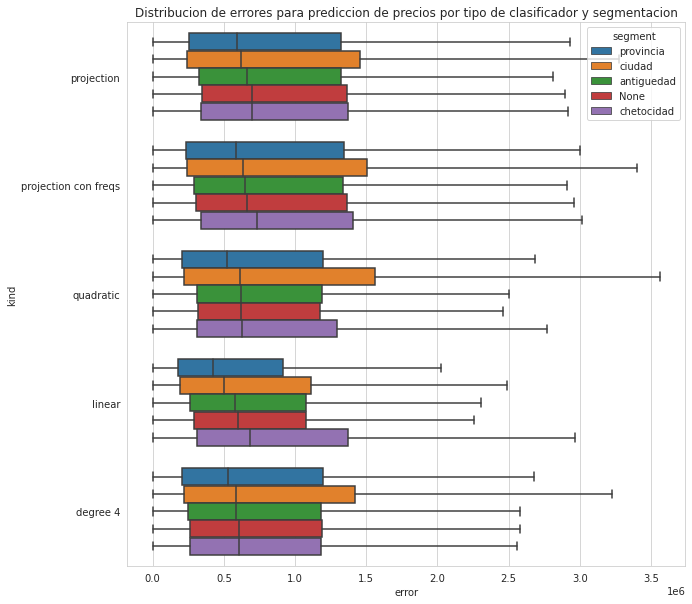
\includegraphics[scale=0.5]{img/cmp/precio/err-by-kind-seg.png}
    \caption{Distribución de errores absolutos cometidos para cada tipo de clasificador por segmento al predecir precio}
    \label{err-precio}
\end{figure}

En \ref{err-precio} se puede ver que ciudad fue el criterio de segmentación que más error tuvo, y curiosamente, si bien chetosidad fue de los mejores para casi todos, en linear fue el que más error tuvo.

\subsection{Metros cubiertos}

\begin{figure}[H]
\centering
\begin{tabular}{ |c|c|c|c|c|c| } 
\hline
\textbf{rank}    & kind    & segment\_by  & r2    & rmse    & rmsle \\ \hline
0   & projection  & tipodepropiedad   & 0.6980 & 51.9076  & 0.2914 \\ \hline
1   & linear  & tipodepropiedad   & 0.6949 & 52.1679  & 0.2967 \\ \hline
2   & quadratic    & tipodepropiedad    & 0.6949  & 52.1679   & 0.2967 \\ \hline
3   & linear  & None  & 0.6288    & 57.5751 & 0.3314 \\ \hline
4   & linear  & antiguedad    & 0.6284  & 57.6881   & 0.3353 \\ \hline
5   & quadratic    & antiguedad & 0.6284   & 57.6881    & 0.3353 \\ \hline
6   & projection  & antiguedad    & 0.6174  & 58.5364   & 0.3476 \\ \hline
7   & projection  & None  & 0.6166    & 58.5094 & 0.3492 \\ \hline
8   & linear  & chetocidad    & 0.5981  & 56.3890   & 0.3369 \\ \hline
9   & quadratic    & chetocidad & 0.5981   & 56.3890    & 0.3369 \\ \hline
10  & projection    & chetocidad   & 0.5832 & 57.4151  & 0.3383 \\ \hline
11  & quadratic  & None  & 0.4090    & 72.6409 & 0.4626 \\ \hline
\end{tabular}
\caption{Resultados por clasificador para la predicción de metros cubiertos}
\label{table:results-m2}
\end{figure}

Como se puede ver, nuestras intuiciones sobre el tipo de propiedad fueron acertadas, ya que los regresores que segmentaban por esta característica ocuparon los primeros puestos en el ranking. Además, los features elegidos fueron buenos, ya que se llegó a casi 0.7 de r2, lo cual indica que es un regresor cercano al ideal, o al menos mucho mas que para precio.

\begin{figure}[H]
    \centering
    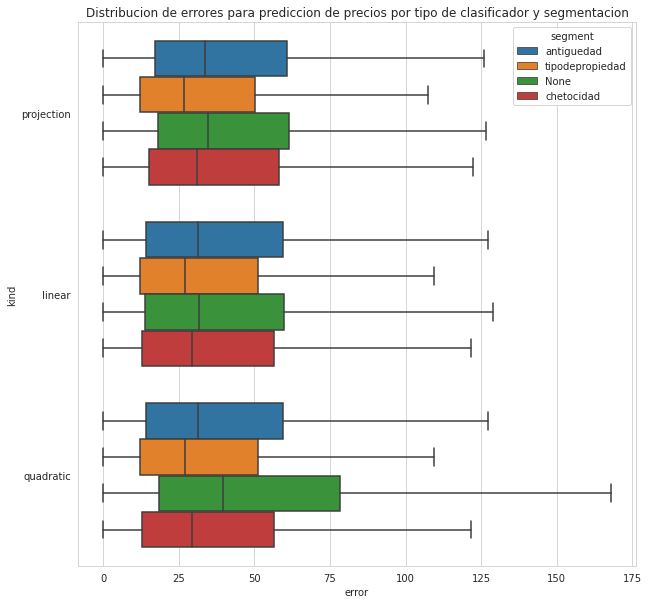
\includegraphics[scale=0.5]{img/cmp/metroscubiertos/err-por-kind-seg.png}
    \caption{Distribución de errores absolutos cometidos para cada tipo de clasificador por segmento al predecir metroscubiertos}
    \label{err-m2}
\end{figure}

En \ref{err-m2} se ve un gráfico del mismo estilo que para precio (fig. \ref{err-precio}). Afortunadamente, en este caso segmentar tendió a ser mejor que no hacerlo, y además, se puede ver como tipodepropiedad es el que menor error tuvo.

\section{Trabajos futuros}

\subsection{Perfeccionando análisis titulo y descripción}

Como se puede ver en los resultados para precio (fig. \ref{table:results-precio}) si bien los resultados obtenidos fueron buenos, nuestro acercamiento a scoring para textos tiene una falla fundamental: es miope frente a palabras diferentes con la misma frecuencia. Por ejemplo, si ``caro" y ``barato" tuvieran frecuencia de 10, dos inmuebles con cada uno como titulo respectivamente tendrian el mismo score, cuando seguramente tengan precios asociados diferentes.

Una forma de remediar esto, es mediante un cambio de enfoque. Utilizar conceptos tomados de NLP, para representar a los textos como vectores en el espacio, y luego de alguna forma dividir ese espacio en embeddings. Finalmente, textos que sean parte del mismo, tenderan a tener características similares aún más profundamente que para nuestro acercamiento. A pesar de que excede el alcance de este trabajo, consideramos interesante comentar la idea.

\subsection{Familias de funciones}

Creemos que construir modelos a través de regresiones por proyección, lineales o polinomiales puede resultar ser suficiente en ciertos problemas, sin embargo, puede no ser así. Puede haber casos donde, lo que se quiere describir presenta comportamientos diferentes a los lineales o polinomiales, por ejemplo, cuando se observa una relación oscilatoria, o logarítmica. A futuro podríamos ver si los precios u otra variable pueden ser modelados por familias de funciones más complejas.

\subsection{Refinamiento del conjunto de datos}

Si bien cuadrados mínimos lineales es un método efectivo a la hora de estimar relaciones entre variables, su efectividad se basa, en gran medida, en que los datos usados a la hora de entrenar el modelo, estén distribuidos de manera favorable. Este supuesto se ve afectado con la aparición de \textit{outliers}. Esto se debe a que el método intenta hacer un balance para minimizar el error de todos los datos, en particular, el de los outliers. Esto en cambio, termina teniendo una gran influencia en las soluciones obtenidas por el método. Una posible avenida para explorar, podría ser el reconocimiento y extracción de estos datos, esperando así, una mejora sustancial en la precisión de nuestros modelos.

%. Para ajustar una recta por ejemplo, se observa que al agregar un outlier, la pendiente de la recta se ve afectada bruscamente, resultando en grandes diferencias entre su valor previo y el nuevo al agregar este dato. Se le llama a este problema "efecto palanca", porque puede verse como, en este caso, la recta se ve atraída hacia este outlier, para compensar los errores. Debido a esto, a nivel practico es posible que una medición que introduce un dato lejos de la realidad, tenga un gran impacto en el resultado final, obteniendo un modelo con una mala calidad de predicción. Por estas razones, es importante identificar estos outliers y removerlos, para minimizar el impacto sobre CML.
    

\section{Conclusión}

En este trabajo, pudimos apreciar las dificultades que se presentan a la hora de diseñar un buen modelo para predecir una variable de un conjunto de datos que no fue \textit{tan} bueno como creíamos. Lo cual nos deja el aprendizaje de que no hay que dar la calidad de los datos por sentado, y siempre hay que analizarlos previo a cualquier entrenamiento.

Asimismo las relaciones entre los fenómenos u observaciones de la vida cotidiana, como pueden ser el precio de inmuebles, no siempre resultan fáciles de analizar. Desde elegir las variables independientes hasta ver sobre que segmentar, se trata de un proceso artesanal, lleno de heurísticas y supuestos. No obstante, no siempre es necesario ahondar en los detalles, y basta con tomar una abstracción tan simple como puede ser una regresión lineal para explicar los datos. Siempre y cuando se hayan segmentado de forma adecuada, con lo cual hay que tener mucho cuidado, de no caer en la trampa que puede ser el \textit{overfitting}. Segmentar demás, tener pocos datos, y que nuestro regresor termine sesgado a los datos de entrenamiento, así realizando predicciones que nada tienen que ver con la realidad.

A pesar de todo esto, en las manos correctas, los regresores junto con CML resultan un método muy poderoso en relación a su complejidad, siendo muy simples. Y tienen la capacidad de  explicar fenómenos complejos presentes en la vida cotidiana de forma satisfactoria.


\begin{thebibliography}{}

\bibitem{islr} 
Gareth James • Daniela Witten • Trevor Hastie
Robert Tibshirani
\textit{
An Introduction to
Statistical Learning
with Applications in R}. 

\end{thebibliography}

\end{document}
